%!TEX root = ../Main.tex
In this section a range of tests will be conducted on different NPG structures in order to uncover the effect of manipulation of the bridges between the Graphene Nano Ribbons (GNR's) in the NPG. From an applied perspective, one of the main motivations is to find out how these bridges can be manipulated in order to control the current through the material. A recent study has shown how one could possibly confine current flow to a single GNR channel by manipulation of bridges between GNR's utilising \textit{Quantum Interference} (QI) effects (See \cref{studyfig2,studyfig3} for some of the results presented in the study). This provides a solution to an important aspect in carbon-based nanocircuitry design, namely confinement of electron flow. The study was focused on the difference in effect of having \textit{meta} and \textit{para} bridges between GNR's. Meta and para bridges are essentially benzene rings oriented in two different ways (more on that in the following sections). The meta and para bridges are 'static' cases in the sense that once made, they are not responsive to any external environment. However, if the bridges are modified with oxygen they become sensitive to f.ex. hydrogenation because of oxygen's tendency to either reduce or oxidise in basic/acidic environments. Thus by hydrogenation it will be possible to tune the electrical properties of the material and make it sensitive to external environments and studies show that hydrogenation of specific sites on nano meter scale is possible experimentally. This section will, in part, be an attempt to reproduce some of the results of the study and to see what happens when oxygen is added to these benzene rings in the meta and para bridges as well as the effects of subsequent hydrogenation of the oxygen.  In \cref{testtable} a schematic overview of the different tests can be seen. The results from these tests will be presented in the form of band structure plots and they will be compared to band structure plots produced with DFT. Additionally a schematic overview of the different systems, showing the on-site potentials of each atom will be presented in the figures as well. Following is a section introducing meta and para NPG in detail. 
\begin{table}[ht]
\begin{tabular}{cclcll}
		\toprule
		Test no. & Meta/Para & Symmetry   & No. of species & Added species & Name  \\ \midrule
		1        & Para      & Symmetric  & 4              & Oxygen        & PS4O  \\
		2        & Para      & Symmetric  & 4              & Hydroxide     & PS4OH \\
		3        & Meta      & Symmetric  & 2              & Oxygen        & MS2O  \\
		4        & Meta      & Symmetric  & 2              & Hydroxide     & MS2OH \\
		5        & Meta      & Asymmetric & 2              & Oxygen        & MA2O  \\
		6        & Meta      & Asymmetric & 2              & Hydroxide     & MA2OH \\
		\bottomrule
	\end{tabular}
	\caption{Table showing an overview of all the structures that will be tested in this section.  How the different species will be manipulated during the tests, will be stated in plots produced for results. The code names follow the table column-wise. In \cref{appfigs}, \cref{Strucow} a collection of figures showing each scenario stated in this table.}
\label{testtable}
\end{table}
\subsection{Differences in para and meta bridges}
In broad terms the difference in the meta and para structures lies in the path an electron will travel through the benzene ring to get across the bridge. In the para bridge, the path across the aromatic ring is symmetric and so the electron will pass above or below with equal probability. Since the para bridge has three bonds in each direction across the ring, the path length in the para bridge is the same on each side (See \cref{studyfig1}). This will cause constructive interference of the states once the waves meet on the other side of the ring, which results in spreading in the density of states from one GNR to the next. For the meta bridge the way across the aromatic ring is not symmetric in the sense that there is two bonds across the path below and four bonds across on the path above (See \cref{studyfig1}). This will cause a shift by half a wavelength between the two paths and thus create destructive interference between waves meeting on the other side of the ring. The effect of this is confinement in the density of states in the GNR's. In \cref{studyfig2} band plots as well as transmission plots are shown for para and meta. In the band plots the two sets of valence/conduction bands around the fermi level shows separation for para and interference for meta. Looking at the transmission plots directly below one can see there is transmission  and thus spreading of the states between the GNR's for para. The area between the two peaks at \SI{0.5}{\electronvolt} and  \SI{1.2}{\electronvolt} show transport between the GNR's. In the transmission plot for meta the transmission is confined. The transmission in the area between the two peaks is pretty much 0. This means that almost no spreading of states occurs between GNR's in meta system. To summarise these results qualitatively: Spreading between the bands in the band plots, corresponds to spreading in the states between the GNR's. Bands on top of each other, showing QI, corresponds to confinement of the states to a single GNR. In the following sections, band plots will mainly be used to show results. Therefore one should keep in mind how they, qualitatively, relate to transmission. In \cref{appfigs}, \cref{allbands} a figure obtained from the developed functions with band plots of normal, para and meta NPG can be seen.
\begin{figure}
    \centering
    \begin{subfigure}[b]{0.48\textwidth}
    \centering
    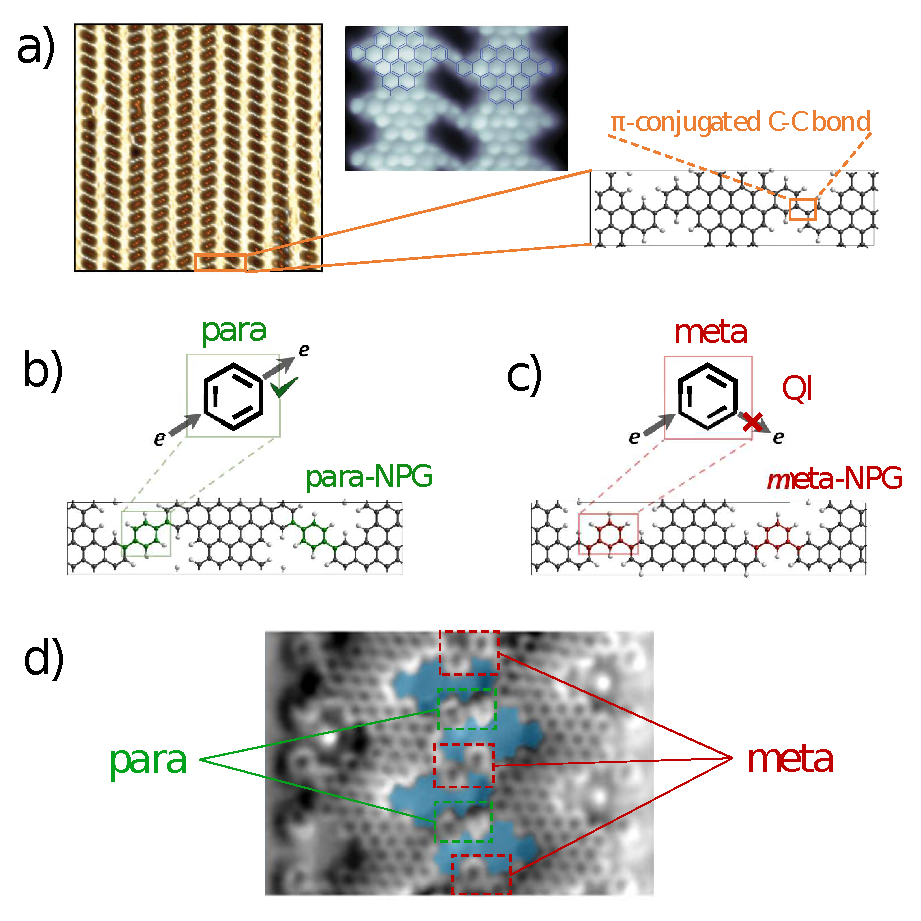
\includegraphics[width=\textwidth]{Figures/Fig_1.eps}
    \caption{Figure showing the some graphical representations of the para and meta bridges (b \& c) as well as some actual pictures taken of NPG showing the bridges (a \& d).}
    \label{studyfig1}
    \end{subfigure}
    ~
    \begin{subfigure}[b]{0.48\textwidth}
    \centering
    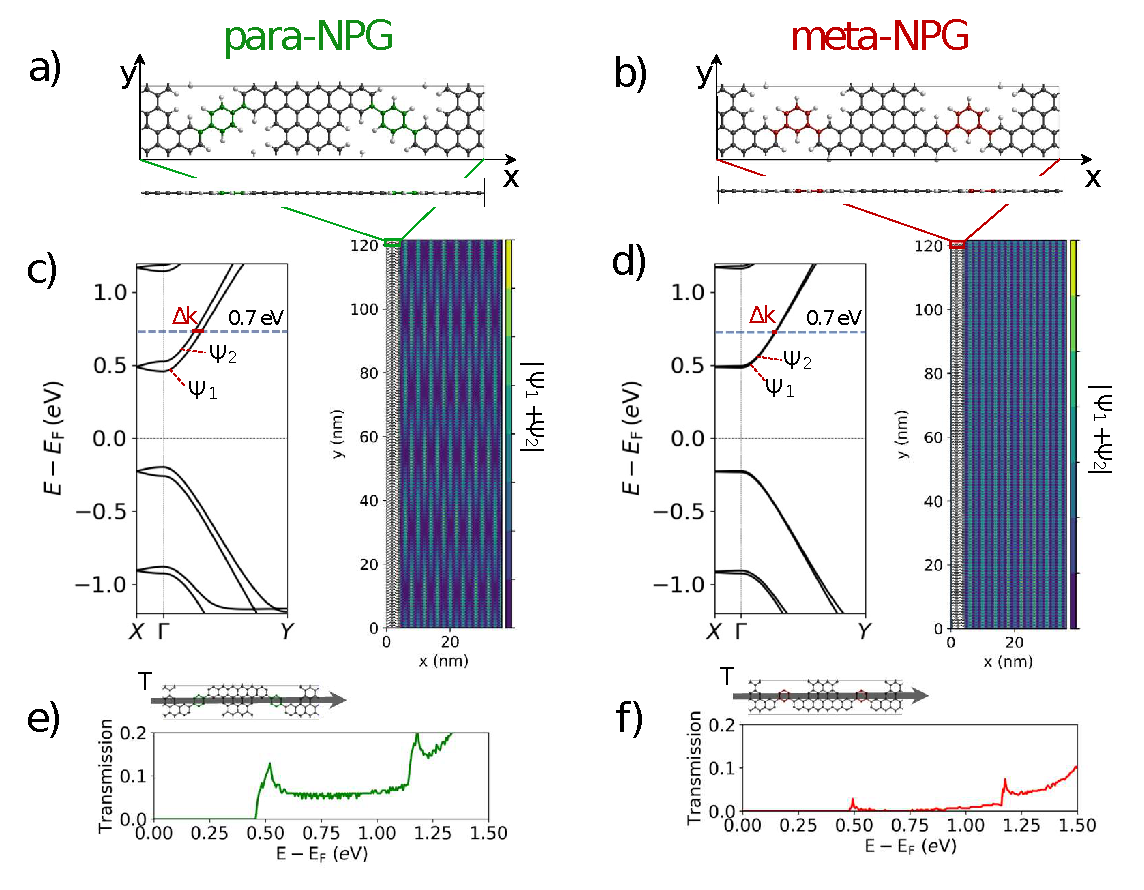
\includegraphics[width=\textwidth]{Figures/Fig_2.eps}
    \caption{Figure showing some band structures (c \& d) and transmission plots (e \& f) from the study obtained with DFT.}
    \label{studyfig2}
    \end{subfigure}
    \vskip\baselineskip
    \begin{subfigure}[b]{0.5\textwidth}
    \centering
    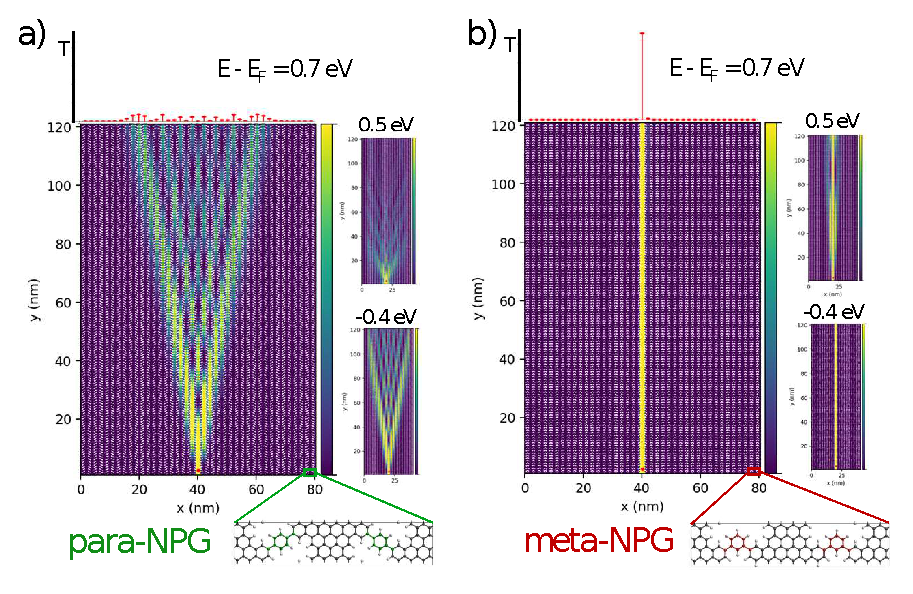
\includegraphics[width = \textwidth]{Figures/Fig_3.eps}
    \caption{Figure showing the currents through the GNR's in a large peace of NPG. Note how the current is spread across GNR's with the para bridge (a) and confined to a single GNR with meta bridge (b).}
    \label{studyfig3}
    \end{subfigure}
    \caption{Figures obtained from [cite] showing both the structures involved as well as some results obtained in the form of band structure and transmission plots.}
    \label{metapara}
\end{figure}
\subsection{Tests with modified meta and para NPG}
The tests consist of three kind of manipulations. Firstly it will be manipulation of the on-site value for the added oxygen atoms (Addition of Oxygen will be simulated by addition of another carbon site to the structure, effectively adding another pi-electron). Secondly simulations of hydrogenation will be done by having added hydroxide groups. By removing hydroxide sites entirely, the aim is to simulate the removal of the extra pi-electron which the oxygen originally provided, but now lost by hydrogenation. Thirdly by manipulation of the on-site potential values of hydroxide, the aim is again to simulate loss of the extra pi-electron. These manipulations will be carried out separately.
\subsection{Test 1: Para-NPG with added oxygen}
The first test will be manipulation of the system 'PS4O'. The basis structure is para-NPG where 4 oxygen sites have been added, two on each benzene ring (see \cref{appfigs}, \cref{Strucow}, no. 5). This is to see the effect of having an extra pi-electron in the system. Practically carbon atoms added instead of oxygen. They will be manipulated by lowering their on-site potential. This is to simulate adding oxygen. In \cref{PS4O} an overview of the system can be seen along with the band structures for the system, obtained through DFT and developed scripts. 
\begin{figure}[h]
    \centering
    \begin{subfigure}[b]{0.3\textwidth}
    \centering
    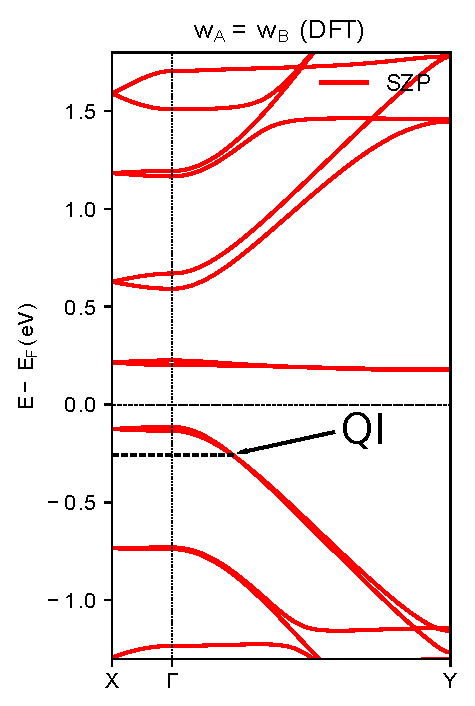
\includegraphics[width=\textwidth]{Figures/PS4ODFT.eps}
    \vspace{-1.5\baselineskip}
    \caption{}
    \label{PS4ODFT}
    \end{subfigure}
    \hspace{20pt}
    \begin{subfigure}[b]{0.3\textwidth}
    \centering
    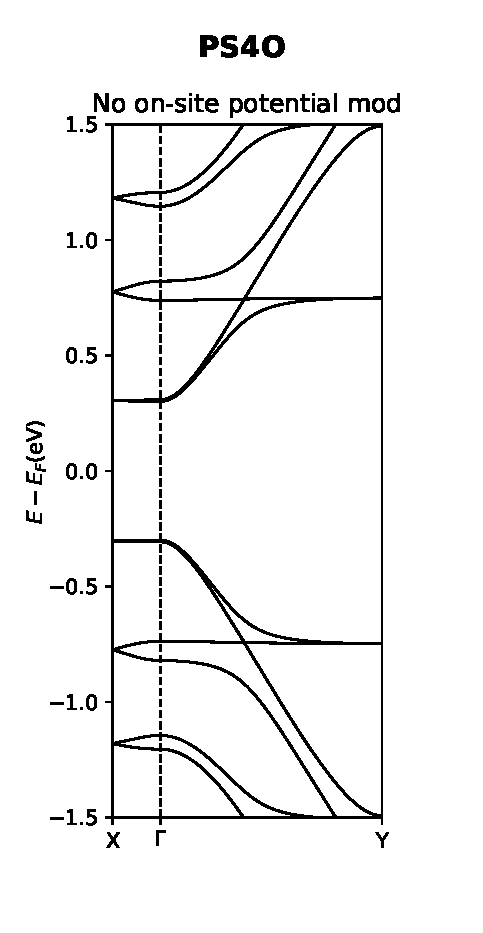
\includegraphics[width=\textwidth]{Figures/PS4Onomod.eps}
    \vspace{-2.5\baselineskip}
    \caption{}
    \label{PS4Odevnomod}
    \end{subfigure}
    ~
    \begin{subfigure}[b]{0.3\textwidth}
    \centering
    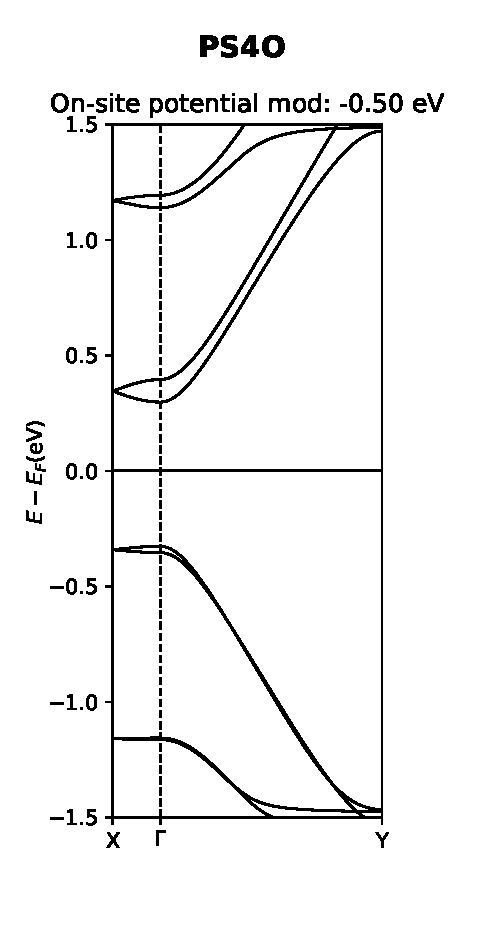
\includegraphics[width=\textwidth]{Figures/PS4Omod.eps}
    \vspace{-2.5\baselineskip}
    \caption{}
    \label{PS4Odevmod}
    \end{subfigure}
    \vskip
    \hspace{4pt}
    \begin{subfigure}[b]{0.8\textwidth}
    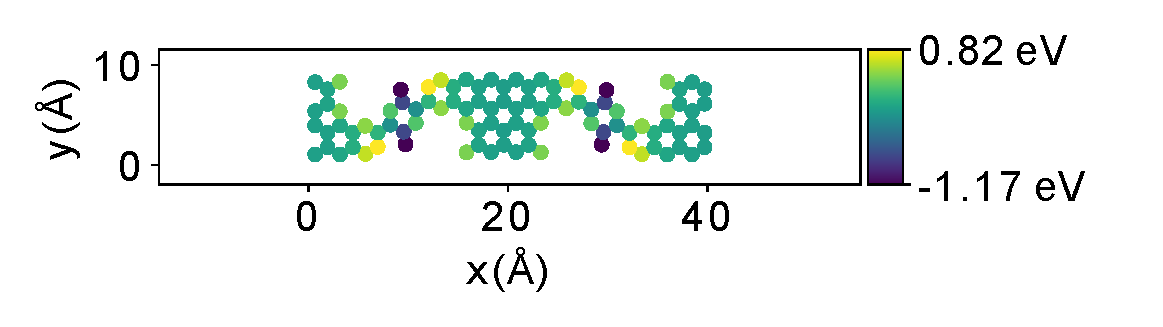
\includegraphics[width=\textwidth]{Figures/PS4O.eps}
    \vspace{-0.5\baselineskip}
    \hspace{-50pt}
    \caption{}
    \label{potmapPS4O}
    \end{subfigure}
    \caption{Figure showing the band structure obtained using DFT a), band structures obtained using developed program with no on-site potential mods b) and with the on-site potential changed to \SI{-0.5}{\electronvolt} c). Lastly a potential map of the system d)}
    \label{PS4O}
\end{figure}
In \cref{PS4Odevnomod,PS4Odevmod} band plots obtained with the developed program is shown. Firstly a band plot without any changes to the on-site potential and next to it a band plot where the on-site potential of the added sites have been changed. As seen \cref{PS4Odevnomod} the band structure produced does not give the right result right away. This is because that the script assumes the same potential everywhere in the system. But as seen on the potential map in \cref{potmapPS4O} especially the potential of the added sites (dark blue) are lower than the rest of the system. To compensate for this, the on-site potential values of those specific sites have been changed by \(\SI{-0.5}{\electronvolt}\) in the script (\cref{PS4Odevmod}) and the result is much closer to that in \cref{PS4ODFT}.
\subsection{Test 2: Simulating hydrogenation of para-NPG with added oxygen atoms}
Next test will be with the 'PS4OH' system. Again the basis structure is para-NPG with added oxygen, but here the aim is to simulate hydrogenation, so therefore the oxygen atoms added will become hydroxide groups. (see \cref{appfigs}, \cref{Strucow}, no. 6). Here the test is to show the difference between removing a OH site entirely (effectively the hydrogen in hydroxide removes the extra pi-electron in oxygen from the system, which can be simulated by removing the atoms entirely) and lowering the on-site potential of the oxygen in the OH group significantly in relation to the rest of the system. Again the results from DTF is shown in \cref{PS4OHDFT} and following the band plots from the developed scripts (\cref{PS4OHremove,PS4OHmod1,PS4OHdevmod2}). 
\begin{figure}[h]
    \centering
    \begin{subfigure}[b]{0.3\textwidth}
    \centering
    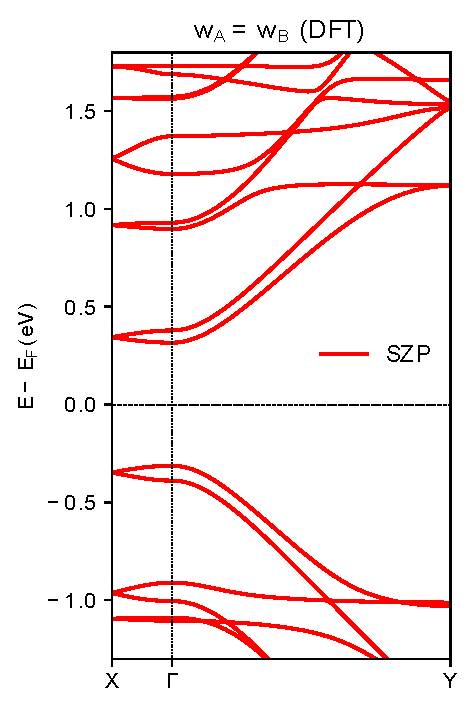
\includegraphics[width=\textwidth]{Figures/PS4OHDFT.eps}
    \vspace{-1.5\baselineskip}
    \caption{}
    \label{PS4OHDFT}
    \end{subfigure}
    \hspace{5pt}
    \begin{subfigure}[b]{0.3\textwidth}
    \centering
    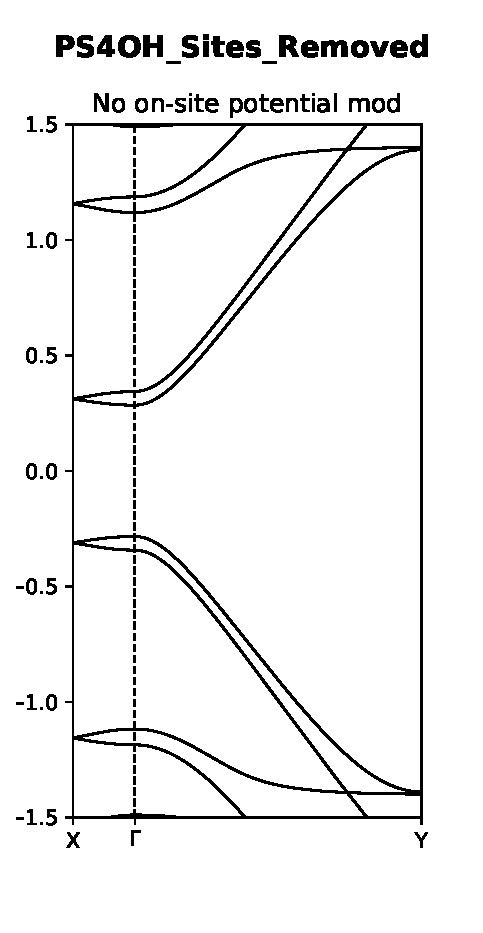
\includegraphics[width=\textwidth]{Figures/PS4OHSitesRemoved.eps}
    \vspace{-2.5\baselineskip}
    \caption{}
    \label{PS4OHremove}
    \end{subfigure}
    \vskip
    \hspace{2pt}
    \begin{subfigure}[b]{0.8\textwidth}
    \centering
    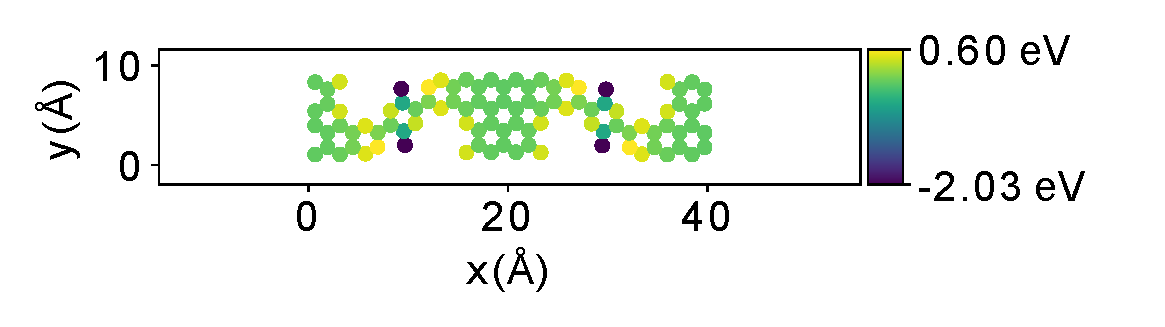
\includegraphics[width=\textwidth]{Figures/PS4OH.eps}
    \vspace{-0.5\baselineskip}
    \hspace{-50pt}
    \caption{}
    \label{potmapPS4OH}
    \end{subfigure}
    \vskip
    \begin{subfigure}[b]{0.3\textwidth}
    \centering
    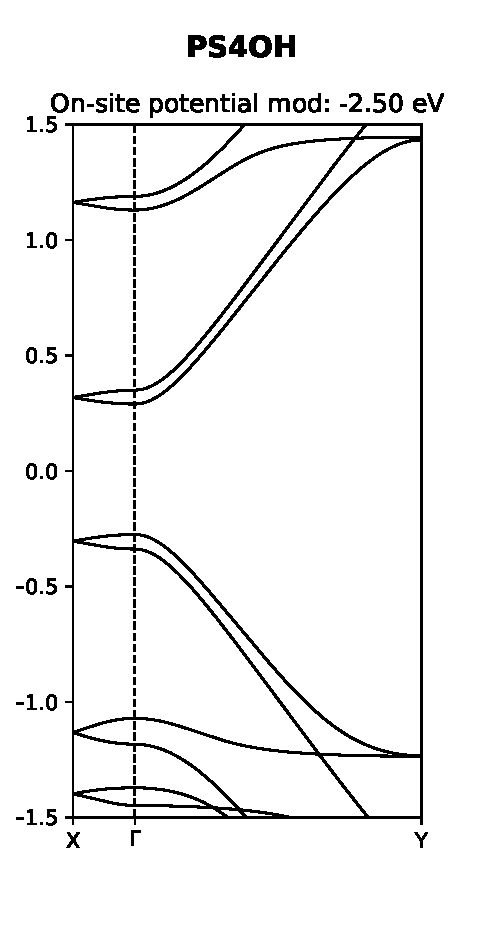
\includegraphics[width=\textwidth]{Figures/PS4OHmod1.eps}
    \vspace{-2.5\baselineskip}
    \caption{}
    \label{PS4OHmod1}
    \end{subfigure}
    ~
    \begin{subfigure}[b]{0.3\textwidth}
    \centering
    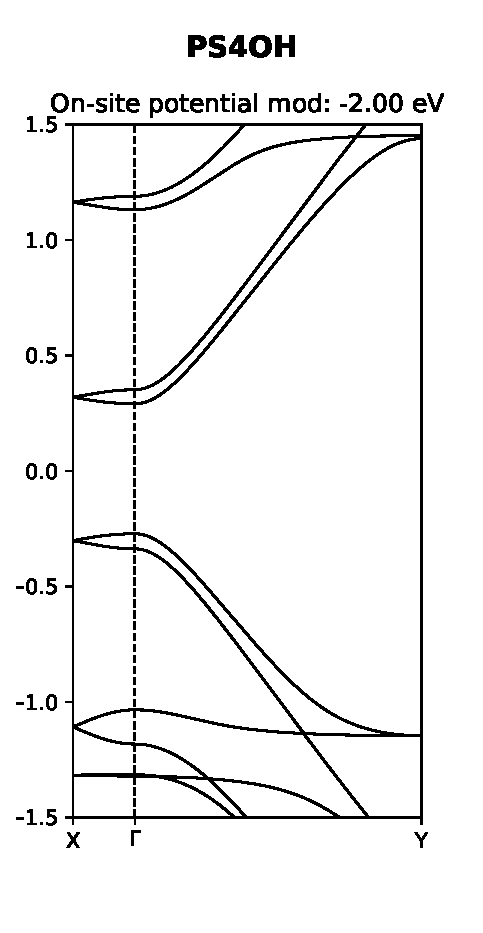
\includegraphics[width=\textwidth]{Figures/PS4OHmod2.eps}
    \vspace{-2.5\baselineskip}
    \caption{}
    \label{PS4OHdevmod2}
    \end{subfigure}
    \caption{Figure showing the band structures obtained using DFT a), band plot where the added sites have been removed b), a potential map of the system c), band plot where the on-site potential has been changed by \SI{-2.5}{\electronvolt} d), and band plot where the on-site potential has been changed by \SI{-2.0}{\electronvolt} e).}
    \label{PS4OH}
\end{figure}
Multiple on-site potentials as well as removal of the specific atomic sites were tested to see which one came closest to that of the band structures in \cref{PS4OHDFT}. The removal was done by removing specific coordinates in the given files before it was run through the script. A seen in \cref{PS4OHremove} the effect of removing the sites gives a plot, somewhat in agreement with \cref{PS4OHDFT}. However the lowest and highest bands does not show. The two other plots in \cref{PS4OHmod1,PS4OHdevmod2} show how gradually changing the on-site potential gets better and better agreement with DFT. A on-site potential of \(\SI{-2.5}{\electronvolt}\) proved to be a bit too high, though still showing good agreement. Lowering the potential to \(\SI{-2.0}{\electronvolt}\) which is the value similar to that given by the lowest potential in the potential map \cref{potmapPS4OH}, yielded a result that is pretty much spot on, considering the valence bands, when compared with DFT. 
\subsection{Test 3}
\subsection{Test 4}
\subsection{Test 5}
\subsection{Test 6}

